% Copyright 2006 by Till Tantau
%
% This file may be distributed and/or modified
%
% 1. under the LaTeX Project Public License and/or
% 2. under the GNU Free Documentation License.
%
% See the file doc/generic/pgf/licenses/LICENSE for more details.


\section{Entity-Relationship Diagram Drawing Library}

\begin{tikzlibrary}{er}
    This packages provides styles for drawing entity-relationship diagrams.
\end{tikzlibrary}
%
\begin{codeexample}[setup code,hidden]
    \usetikzlibrary{er}
\end{codeexample}

This library is intended to help you in creating E/R-diagrams. It defines only
few new styles, but using the style |entity| instead of saying |rectangle,draw|
makes the code more expressive.


\subsection{Entities}

The package defines a simple style for drawing entities:

\begin{stylekey}{/tikz/entity}
    This style is to be used with nodes that represent entity types. It causes
    the node's shape to be set to a rectangle that is drawn and whose minimum
    size and width are set to sensible values.

    Note that this style is called |entity| despite the fact that it is to be
    used for nodes representing entity \emph{types} (the difference between an
    entity and an entity type is the same as the difference between an object
    and a class in object-oriented programming). If this bothers you, feel free
    to define a style |entity type| instead.
    %
\begin{codeexample}[preamble={\usetikzlibrary{positioning}}]
\begin{tikzpicture}
  \node[entity] (sheep)                   {Sheep};
  \node[entity] (genome) [right=of sheep] {Genome};
\end{tikzpicture}
\end{codeexample}
    %
\end{stylekey}

\begin{stylekey}{/tikz/every entity}
    This style is evoked by the style |entity|. To change the appearance of
    entities, you can change this style.
    %
\begin{codeexample}[preamble={\usetikzlibrary{positioning}}]
\begin{tikzpicture}
  [every entity/.style={draw=blue!50,fill=blue!20,thick}]
  \node[entity] (sheep)                   {Sheep};
  \node[entity] (genome) [right=of sheep] {Genome};
\end{tikzpicture}
\end{codeexample}
    %
\end{stylekey}


\subsection{Relationships}

Relationships are drawn using styles that are very similar to the styles for
entities.

\begin{stylekey}{/tikz/relationship}
    This style works like |entity|, only it is to be used for relationships.
    Again, |relationship|s are actually relationship types.
    %
\begin{codeexample}[]
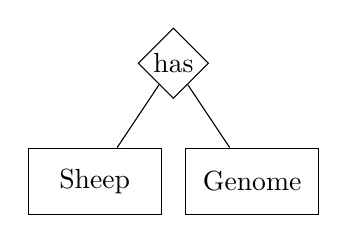
\begin{tikzpicture}
  \node[entity] (sheep)  at (0,0)   {Sheep};
  \node[entity] (genome) at (2,0)   {Genome};
  \node[relationship]    at (1,1.5) {has}
    edge (sheep)
    edge (genome);
\end{tikzpicture}
\end{codeexample}
    %
\end{stylekey}

\begin{stylekey}{/tikz/every relationship}
    Works like |every entity|.
    %
\begin{codeexample}[]
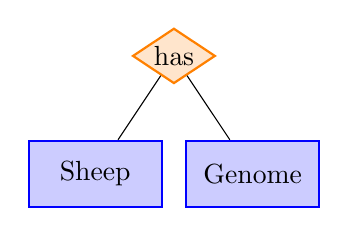
\begin{tikzpicture}
  [every entity/.style={fill=blue!20,draw=blue,thick},
   every relationship/.style={fill=orange!20,draw=orange,thick,aspect=1.5}]
  \node[entity] (sheep)  at (0,0)   {Sheep};
  \node[entity] (genome) at (2,0)   {Genome};
  \node[relationship]    at (1,1.5) {has}
    edge (sheep)
    edge (genome);
\end{tikzpicture}
\end{codeexample}
    %
\end{stylekey}


\subsection{Attributes}

\begin{stylekey}{/tikz/attribute}
    This style is used to indicate that a node is an attribute. To connect an
    attribute to its entity, you can use, for example, the |child| command or
    the |pin| option.
    %
\begin{codeexample}[]
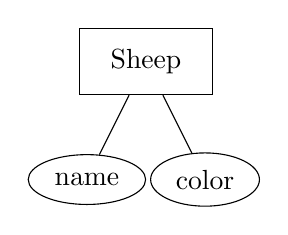
\begin{tikzpicture}
  \node[entity] (sheep)  {Sheep}
    child {node[attribute] {name}}
    child {node[attribute] {color}};
\end{tikzpicture}
\end{codeexample}
    %
\begin{codeexample}[]
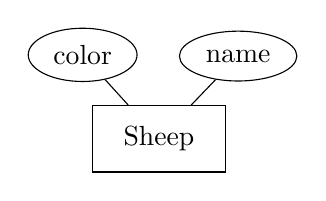
\begin{tikzpicture}[every pin edge/.style=draw]
  \node[entity,pin={[attribute]60:name},pin={[attribute]120:color}] {Sheep};
\end{tikzpicture}
\end{codeexample}
    %
\end{stylekey}

\begin{stylekey}{/tikz/key attribute}
    This style is intended for key attributes. By default, the will cause the
    attribute to be typeset in italics. Typically, underlining is used instead,
    but that looks ugly and it is difficult to implement in \TeX.
\end{stylekey}

\begin{stylekey}{/tikz/every attribute}
    This style is used with every attribute, and therefore also for every key
    attribute.
    %
\begin{codeexample}[]
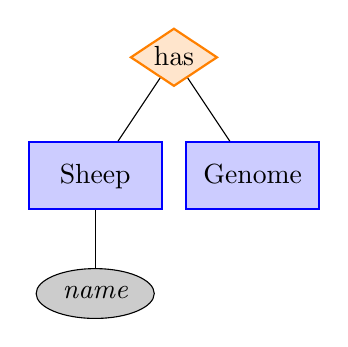
\begin{tikzpicture}
  [text depth=1pt,
   every attribute/.style={fill=black!20,draw=black},
   every entity/.style={fill=blue!20,draw=blue,thick},
   every relationship/.style={fill=orange!20,draw=orange,thick,aspect=1.5}]

  \node[entity] (sheep)  at (0,0)   {Sheep}
    child {node  [key attribute] {name}};
  \node[entity] (genome) at (2,0)   {Genome};
  \node[relationship]    at (1,1.5) {has}
    edge (sheep)
    edge (genome);
\end{tikzpicture}
\end{codeexample}
    %
\end{stylekey}


%%% Local Variables:
%%% mode: latex
%%% TeX-master: "pgfmanual-pdftex-version"
%%% End:
